\documentclass[conference]{IEEEtran}
\usepackage{times}
\usepackage[numbers]{natbib}
\usepackage{multicol}
\usepackage{amsmath,amssymb,amsfonts}
\usepackage{graphicx}
\usepackage{booktabs}
\usepackage{tabularx}
\usepackage{multirow}
\usepackage{microtype}
\let\labelindent\relax
\usepackage{enumitem}
\setlist{noitemsep, topsep=1.5pt, leftmargin=*}
\usepackage{xcolor}
\usepackage{tikz}
\usetikzlibrary{shapes.geometric, arrows.meta, positioning, calc, backgrounds, fit}
\usepackage[bookmarks=true,hidelinks]{hyperref}

% Define color palette
\definecolor{brandblue}{RGB}{31, 78, 121}
\definecolor{brandred}{RGB}{192, 0, 0}
\definecolor{brandgreen}{RGB}{56, 124, 68}
\definecolor{brandamber}{RGB}{197, 90, 17}
\definecolor{brandpurple}{RGB}{112, 48, 160}
\definecolor{brandteal}{RGB}{0, 128, 128}
\definecolor{brandslate}{RGB}{80, 80, 80}
\definecolor{boxbg}{RGB}{245, 247, 250}

\pdfinfo{
   /Author (Anonymous)
   /Title  (AFFORD-Bench: An Affordance-Grounded Benchmark and Generalization Evaluation for Robot Learning)
   /Subject (Robotics Benchmarks, Imitation Learning, Out-of-Distribution Generalization, Affordance Grounding)
   /Keywords (Robot Manipulation; Vision-Language-Action Models; Affordance Grounding; Out-of-Distribution Benchmark)
}

\begin{document}

\title{AFFORD-Bench: An Affordance-Grounded Benchmark and Generalization Evaluation for Robot Learning}

\author{Author Names Omitted for Anonymous Review. Paper-ID [RSS-2027-0150]}

\maketitle

\begin{abstract}
Imitation learning policies and Vision-Language-Action (VLA) models have demonstrated remarkable empirical success in robotic manipulation. However, recent benchmark analyses, such as LIBERO-PRO and LIBERO-X, have uncovered a fundamental crisis in evaluation: high task completion rates frequently collapse under even minor environmental perturbations, exposing policies that rely on rote trajectory memorization rather than genuine environmental comprehension. Crucially, existing benchmarks evaluate distribution shifts predominantly in narrow tabletop settings using superficial appearance or instruction variations, ignoring physical affordances---contact mechanics, kinematic clearances, dynamic friction, and compliance---that govern physical interaction. In this paper, we introduce \textbf{AFFORD-Bench}, a large-scale, affordance-grounded manipulation benchmark spanning \textbf{210 diverse physical tasks} across \textbf{7 distinct domains}: Industrial Precision, Culinary Operations, Domestic Tabletop, Cleanroom Laboratory Sciences, Long-Horizon Multi-Stage Sequences, Multi-Stage Precision Chaining, and Sequential Service \& Culinary Assembly. Operating in a high-fidelity Franka Emika Panda simulation environment, AFFORD-Bench provides 10,500 expert demonstrations across dual-camera high-resolution RGB ($640\times 660$ workcell and $300\times 420$ wrist) alongside aligned 3D metric depth and 7-DoF impedance states ($>2.2\times 10^6$ physical timesteps). We formalize a systematic combinatorial perturbation manifold spanning Spatial-Kinematic ($\pm \Delta \mathbf{p}$, orientation tilts, insertion tolerances), Physical-Dynamic (Coulomb friction $\mu \in [0.1, 1.2]$, mass scaling $0.5\times$--$3.0\times$), and Visual-Photometric axes across 35 benchmark evaluation suites. We introduce compound multi-subtask prompts chaining 2--3 sequential actions in single continuous instructions. We detail standardized training and evaluation protocols, establishing metrics including the Physical Robustness Index (PRI) and Generalization Degradation Index (GDI). Our empirical evaluations across leading policy representations---including Diffusion Policy, ACT, OpenVLA-7B, SmolVLA-450M, and AtomVLA---demonstrate that state-of-the-art architectures degrade non-uniformly along affordance boundaries, confirming that physical affordance grounding is necessary for generalizable manipulation.
\end{abstract}

\IEEEpeerreviewmaketitle

\section{Introduction}
\label{sec:intro}

The field of robot learning is undergoing a profound paradigm shift driven by the emergence of generalist Vision-Language-Action (VLA) models~\cite{kim2024openvla, octo2023, padalkar2023openx}, compact edge architectures such as SmolVLA~\cite{smolvla2025}, subtask-aware post-training frameworks like AtomVLA~\cite{atomvla2025}, and expressive visuomotor policies~\cite{chi2023diffusion, zhao2023act}. By unifying multi-modal perception with end-to-end motor control, these architectures promise to endow robotic manipulators with cross-task generalization and zero-shot adaptability. 

However, measuring whether these models exhibit true physical generalizability remains an acute open challenge. Standardized evaluation suites such as LIBERO~\cite{liu2023libero} have become the de facto testing ground for policy comparison. Yet, rigorous post-hoc investigations by \citet{zhou2026liberopro} (LIBERO-PRO) and \citet{wang2026liberox} (LIBERO-X) revealed that the seemingly high success rates reported on standard benchmarks are severely inflated. When subjected to minor spatial offsets or altered visual conditions, policies that previously achieved over 90\% success suffer catastrophic degradation down to near 0\%. As established in both analyses, current models overfit to rote trajectory memorization and nominal scene layouts from demonstration data, lacking any grounded understanding of task goals.

\begin{figure}[t]
\centering
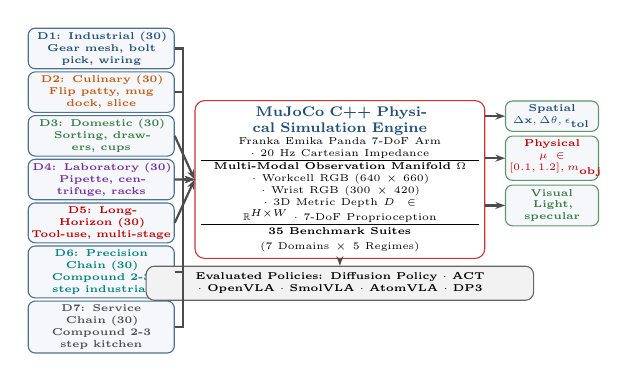
\begin{tikzpicture}[
    scale=0.72, every node/.style={transform shape},
    domainbox/.style={rectangle, rounded corners=2.5pt, draw=brandblue!80, fill=boxbg, inner sep=1.8pt, text width=2.45cm, align=center, font=\tiny\bfseries},
    corebox/.style={rectangle, rounded corners=3.5pt, draw=brandred!80, fill=white, inner sep=3.0pt, text width=4.9cm, align=center, font=\scriptsize},
    axisbox/.style={rectangle, rounded corners=2.5pt, draw=brandgreen!80, fill=boxbg, inner sep=2.0pt, text width=1.5cm, align=center, font=\tiny\bfseries},
    arr/.style={-{Stealth[length=3.5pt,width=2.5pt]}, thick, draw=black!70}
]
    % Domains column (7 domains)
    \node[domainbox] (d1) {\color{brandblue}D1: Industrial (30)\\ \tiny Gear mesh, bolt pick, wiring};
    \node[domainbox, below=1.2pt of d1] (d2) {\color{brandamber}D2: Culinary (30)\\ \tiny Flip patty, mug dock, slice};
    \node[domainbox, below=1.2pt of d2] (d3) {\color{brandgreen}D3: Domestic (30)\\ \tiny Sorting, drawers, cups};
    \node[domainbox, below=1.2pt of d3] (d4) {\color{brandpurple}D4: Laboratory (30)\\ \tiny Pipette, centrifuge, racks};
    \node[domainbox, below=1.2pt of d4] (d5) {\color{brandred}D5: Long-Horizon (30)\\ \tiny Tool-use, multi-stage};
    \node[domainbox, below=1.2pt of d5] (d6) {\color{brandteal}D6: Precision Chain (30)\\ \tiny Compound 2-3 step industrial};
    \node[domainbox, below=1.2pt of d6] (d7) {\color{brandslate}D7: Service Chain (30)\\ \tiny Compound 2-3 step kitchen};

    % Core Engine (aligned with middle domain D4)
    \node[corebox, right=10pt of d4] (sim) {
        \textbf{\color{brandblue}MuJoCo C++ Physical Simulation Engine}\\
        \tiny Franka Emika Panda 7-DoF Arm $\cdot$ 20 Hz Cartesian Impedance\\
        \vspace{1pt}\hrule\vspace{1pt}
        \textbf{Multi-Modal Observation Manifold $\Omega$}\\
        $\cdot$ Workcell RGB ($640\times 660$) $\cdot$ Wrist RGB ($300\times 420$)\\
        $\cdot$ 3D Metric Depth $D \in \mathbb{R}^{H\times W}$ $\cdot$ 7-DoF Proprioception\\
        \vspace{1pt}\hrule\vspace{1pt}
        \textbf{35 Benchmark Suites} ($7 \text{ Domains} \times 5 \text{ Regimes}$)
    };

    % Perturbation axes
    \node[axisbox, right=10pt of sim.north east, yshift=-8pt] (p_spat) {\color{brandblue}Spatial\\ \tiny $\Delta \mathbf{x}, \Delta\theta, \epsilon_{\text{tol}}$};
    \node[axisbox, below=2pt of p_spat] (p_phys) {\color{brandred}Physical\\ \tiny $\mu \in [0.1, 1.2], m_{\text{obj}}$};
    \node[axisbox, below=2pt of p_phys] (p_vis) {\color{brandgreen}Visual\\ \tiny Light, specular};

    % Policy baselines
    \node[rectangle, rounded corners=3pt, draw=black!60, fill=gray!10, text width=6.6cm, align=center, font=\tiny\bfseries, below=3.5pt of sim] (policy) {
        Evaluated Policies: Diffusion Policy $\cdot$ ACT $\cdot$ OpenVLA $\cdot$ SmolVLA $\cdot$ AtomVLA $\cdot$ DP3
    };

    % Connectors
    \draw[arr] (d1.east) -- ++(4pt,0) |- (sim.west);
    \draw[arr] (d2.east) -- ++(4pt,0) |- (sim.west);
    \draw[arr] (d3.east) -- (sim.west);
    \draw[arr] (d4.east) -- (sim.west);
    \draw[arr] (d5.east) -- (sim.west);
    \draw[arr] (d6.east) -- ++(4pt,0) |- (sim.west);
    \draw[arr] (d7.east) -- ++(4pt,0) |- (sim.west);

    \draw[arr] (sim.east |- p_spat) -- (p_spat.west);
    \draw[arr] (sim.east |- p_phys) -- (p_phys.west);
    \draw[arr] (sim.east |- p_vis) -- (p_vis.west);

    \draw[arr] (sim.south) -- (policy.north);
\end{tikzpicture}
\caption{\textbf{The AFFORD-Bench Architecture.} Spanning 210 tasks across 7 distinct domains, benchmarking out-of-distribution generalization across Spatial-Kinematic, Physical-Dynamic, and Visual-Photometric shifts in 35 standardized evaluation suites.}
\label{fig:teaser}
\end{figure}

While LIBERO-PRO and LIBERO-X took vital steps by introducing independent and hierarchical perturbations, existing benchmarks remain constrained by a critical limitation: \textbf{the absence of physical affordance grounding}. In ecological psychology and robotics~\cite{gibson1979ecological}, an \textit{affordance} defines actionable properties between an agent and its physical environment. Real-world robotic manipulation is not merely a geometric or visual alignment problem; it is fundamentally governed by contact mechanics, surface friction, kinematic compliance, mass distributions, and tight clearance tolerances. In existing suites, tasks are largely limited to unconstrained tabletop pick-and-place operations in toy domestic scenes, where collisions and contact physics are trivialized. Consequently, they fail to evaluate whether a policy can adapt to variations in physical contact constraints (e.g., insertion resistance, grasping friction, pipette liquid aspiration, or high-tolerance gear meshing).

To bridge this foundational gap, this paper introduces \textbf{AFFORD-Bench}, an affordance-grounded benchmark designed to expose the boundary between visual memorization and physical generalizability. AFFORD-Bench advances robot learning along four primary axes:
\begin{enumerate}
    \item \textbf{Scale and Domain Diversity}: We formulate \textbf{210 distinct physical manipulation tasks} across \textbf{7 specialized domains}: Industrial Precision, Culinary Operations, Domestic Tabletop, Cleanroom Laboratory Sciences, Long-Horizon Multi-Stage Sequences, Multi-Stage Precision Chaining, and Sequential Service \& Culinary Assembly.
    \item \textbf{Multi-Subtask Prompt Composition}: Analogous to multi-step execution in long-horizon robotics, domains D6 and D7 introduce compound natural language instructions chaining 2--3 sequential subtasks (e.g., ``align shaft, press bearing, and lock clamp''), evaluating whether policies can sustain affordance alignment under cumulative compounding errors.
    \item \textbf{Affordance-Grounded Perturbation Space}: Unlike prior benchmarks that alter visual textures or object coordinates in isolation, we formalize a structured perturbation manifold across three orthogonal physical axes: \textit{Spatial-Kinematic} (clearance tolerances $\pm 1.5\,\text{mm}$ to $\pm 10\,\text{mm}$, orientation tilts), \textit{Physical-Dynamic} (Coulomb friction $\mu \in [0.1, 1.2]$, object masses $0.5\times$ to $3.0\times$, contact damping), and \textit{Visual-Photometric} (lighting angle, specularity, distractor clutter), yielding \textbf{35 standardized benchmark evaluation suites}.
    \item \textbf{High-Throughput, Zero-Cost Reproducibility}: Using native C++ MuJoCo physics~\cite{todorov2012mujoco}, we synthesize 10,500 expert demonstrations (50 per task, $>2.2\times 10^6$ timesteps) via deterministic algorithmic oracles running at 40--50 FPS with zero external API costs. Datasets are packaged in standardized Robomimic/HDF5 format directly compatible with Diffusion Policy, ACT, OpenVLA, SmolVLA, AtomVLA, and Octo.
\end{enumerate}

\begin{figure*}[t]
\centering
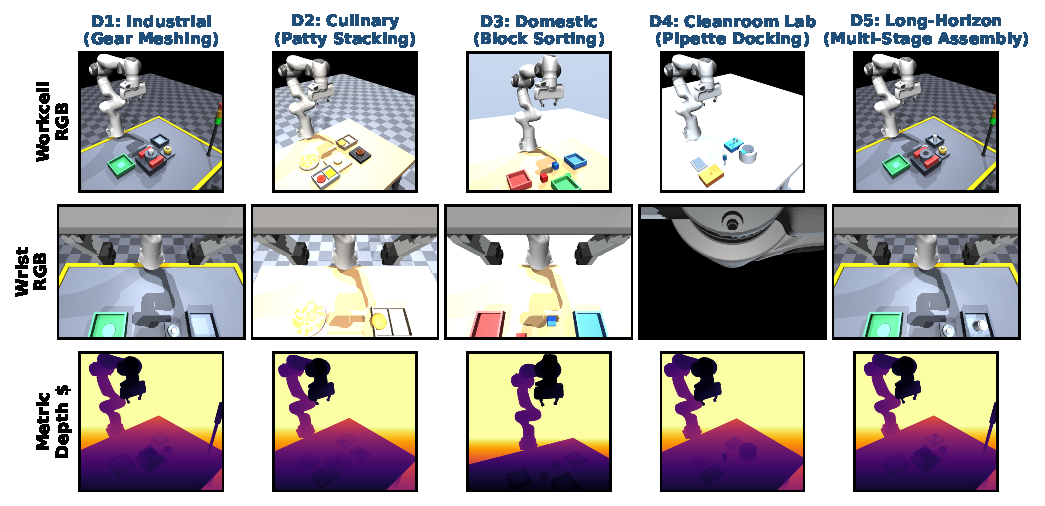
\includegraphics[width=\linewidth, height=3.4cm]{figures/tasks_horizontal_vis.pdf}
\caption{\textbf{Multi-Domain Qualitative Visualizations in AFFORD-Bench.} Synchronized multi-modal observations across representative tasks from all seven benchmark domains: (Row 1) Third-person workcell visual stream ($640\times 660$ RGB); (Row 2) Wrist-mounted eye-in-hand visual stream ($300\times 420$ RGB); (Row 3) Aligned 3D metric depth maps ($D_{3D}$, colored by physical meter distance). Spans industrial precision assembly (D1), commercial culinary operations (D2), domestic block sorting (D3), cleanroom pharmaceutical sciences (D4), long-horizon tool assembly (D5), multi-stage precision chaining (D6), and sequential culinary assembly (D7).}
\label{fig:tasks_vis}
\end{figure*}

\section{Related Work}
\label{sec:related}

\subsection{Robotic Manipulation Benchmarks}
Benchmarking in robotic manipulation has evolved from single-domain suites to diverse simulation platforms. RLBench~\cite{james2020rlbench} and ManiSkill2~\cite{gu2023maniskill2} provided simulation suites for reinforcement learning and demonstration-guided policy learning. Robomimic~\cite{mandlekar2021robomimic} established standardized offline imitation learning pipelines and empirical evaluation protocols across varied human demonstration qualities. LIBERO~\cite{liu2023libero} introduced a 130-task suite structured around knowledge transfer in lifelong learning, evaluating sequential task acquisition. However, all these suites focus primarily on nominal execution without systematic physical out-of-distribution (OOD) testing.

\subsection{OOD Robustness and Modern VLA Architectures}
With the proliferation of large-scale pretrained models~\cite{padalkar2023openx, brohan2022rt1, brohan2023rt2, kim2024openvla, octo2023}, assessing policy robustness against distribution shifts has become critical. \citet{zhou2026liberopro} established LIBERO-PRO, illustrating that state-of-the-art policies achieve high success under nominal LIBERO conditions but collapse when subject to perturbed objects, initial states, or paraphrased instructions. Building on this, \citet{wang2026liberox} introduced LIBERO-X, demonstrating that prior benchmarks fail to evaluate compounded distribution shifts across hierarchical difficulty levels. Concurrently, the community has pushed toward efficient edge-deployable VLAs like \textbf{SmolVLA}~\cite{smolvla2025}, which utilizes a compact 450M parameter vision-language backbone with a flow-matching action expert to drastically reduce inference latency, and \textbf{AtomVLA}~\cite{atomvla2025}, which introduces atomic subtask decomposition paired with a predictive world model to mitigate error accumulation in long-horizon tasks. However, existing benchmarks evaluate these modern architectures primarily within standard domestic tabletop scenes, failing to probe contact dynamics, surface friction, or precision assembly.

\subsection{Affordance and Visuomotor Policy Learning}
Affordance theory~\cite{gibson1979ecological} posits that agents perceive objects in terms of potential physical interactions. In robotics, affordance-guided manipulation has been explored via contact-rich grasping~\cite{song2023grasping}, spatial affordance maps~\cite{shridhar2022cliport}, and explicit 3D representations such as 3D Diffusion Policy (DP3)~\cite{ze2024dp3}. While Diffusion Policy~\cite{chi2023diffusion} and Action Chunking with Transformers (ACT)~\cite{zhao2023act} achieve high tracking precision on low-cost hardware~\cite{fu2024mobilealoha}, their ability to generalize across physical affordance shifts remains uncharacterized at scale. AFFORD-Bench provides the first systematic benchmark unifying multi-domain manipulation with explicit affordance-space perturbation manifolds.

\section{The AFFORD-Bench Benchmark}
\label{sec:benchmark}

\subsection{Task Formulation as Affordance-Constrained MDPs}
We formalize each manipulation task as an Affordance-Constrained Markov Decision Process defined by the tuple $\mathcal{M} = \langle \mathcal{S}, \mathcal{A}, \mathcal{T}, \mathcal{R}, \Omega, \mathcal{C}_{\text{aff}} \rangle$, where $\mathcal{S}$ is the continuous state space of the robot and environment, $\mathcal{A} \subset \mathbb{R}^4$ is the action space representing 3D Cartesian end-effector delta velocity $\Delta \mathbf{x} \in \mathbb{R}^3$ and continuous gripper command $a_{\text{grip}} \in [-1, 1]$, $\mathcal{T}(s' \mid s, a)$ is the transition probability governed by MuJoCo multi-body contact dynamics, and $\mathcal{R}(s, a) \in \{0, 1\}$ is a sparse task completion indicator. 

Crucially, $\mathcal{C}_{\text{aff}} \subset \mathcal{S} \times \mathcal{A}$ denotes the \textit{affordance constraint set}. For a task to be successfully executed, the state trajectory must satisfy both geometric tolerances and dynamic contact stability:
\begin{align}
\mathcal{C}_{\text{aff}} = \Big\{ (s, a) \;\Big|\;& \|\mathbf{p}_{\text{obj}} - \mathbf{p}_{\text{goal}}\|_{\mathbf{W}} \le \epsilon_{\text{tol}}, \notag \\
& F_{\text{contact}} \le F_{\max}, \; \frac{F_{\text{friction}}}{F_{\text{normal}}} \le \mu \Big\},
\end{align}
where $\mathbf{W} = \text{diag}(w_x, w_y, w_z)$ weights directional tolerance, $\epsilon_{\text{tol}}$ represents insertion or placement threshold, and $\mu$ is Coulomb friction.

\begin{table*}[t]
\centering
\caption{\textbf{Comprehensive Taxonomy of the AFFORD-Bench Suite.} Spanning 210 formally defined physical tasks across 7 distinct domains, featuring diverse kinematic constraints, contact dynamics, and clearance tolerances across 35 benchmark evaluation suites.}
\label{tab:domains}
\scriptsize
\setlength{\tabcolsep}{2.5pt}
\renewcommand{\arraystretch}{0.91}
\begin{tabularx}{\linewidth}{lccXcX}
\toprule
\textbf{Domain} & \textbf{Task IDs} & \textbf{Count} & \textbf{Representative Manipulation Tasks} & \textbf{Clearance ($\epsilon$)} & \textbf{Dominant Contact Physics} \\
\midrule
\textbf{D1: Industrial Precision} & 001--030 & 30 & Gear meshing, bolt insertion, cable routing, fixture latching & $\pm 2.0\text{--}5.0\,\text{mm}$ & High stiffness, rigid peg-in-hole friction \\
\textbf{D2: Culinary Operations} & 031--060 & 30 & Patty flipping, espresso mug docking, slicing alignment, pouring & $\pm 5.0\text{--}12.0\,\text{mm}$ & Deformable contact, non-planar slipping \\
\textbf{D3: Domestic Tabletop} & 061--090 & 30 & Color block sorting, drawer opening, stack packing, cup nesting & $\pm 8.0\text{--}20.0\,\text{mm}$ & Multi-body clutter, dynamic toppling \\
\textbf{D4: Laboratory Sciences} & 091--120 & 30 & Pipette tip pickup, centrifuge vial docking, reagent mixing & $\pm 1.5\text{--}4.0\,\text{mm}$ & Precision alignment, fragile glass contact \\
\textbf{D5: Long-Horizon Sequences} & 121--150 & 30 & Multi-stage assembly, tool-assisted latching, sequential routing & $\pm 3.0\text{--}10.0\,\text{mm}$ & Cumulative error accumulation, sub-goal chaining \\
\textbf{D6: Precision Chaining} & 151--180 & 30 & Shaft-bearing-clamp, gasket-bolt-torque, terminal-wire-seal & $\pm 1.8\text{--}4.5\,\text{mm}$ & Compounded insertion tolerances, high torque \\
\textbf{D7: Service Assembly} & 181--210 & 30 & Burger patty-cheese-bun, mug-brew-serve, plate-fork-napkin & $\pm 4.0\text{--}10.0\,\text{mm}$ & Dynamic re-grasping, multi-stage compliance \\
\midrule
\textbf{Total Benchmark Scope} & \textbf{001--210} & \textbf{210} & \textbf{7 Domains $\times$ 30 Tasks = 210 Tasks (35 Evaluation Suites)} & $\pm 1.5\text{--}20.0\,\text{mm}$ & \textbf{10,500 Demonstrations ($>2.2\times 10^6$ Steps)} \\
\bottomrule
\end{tabularx}
\end{table*}

\subsection{Domain Architecture}
As summarized in Table~\ref{tab:domains} and visualized in Figure~\ref{fig:tasks_vis}, AFFORD-Bench is partitioned into seven specialized domains, each comprising 30 distinct tasks:
\textbf{D1: Industrial Precision} (Tasks 001--030) targets assembly-line operations requiring sub-centimeter accuracy, including gear meshing onto splined shafts, flange bolt insertion, cable routing, and toggle clamps.
\textbf{D2: Culinary Operations} (Tasks 031--060) simulates commercial kitchen preparation, including spatula patty flips, espresso mug docking, ingredient transfer, and sanitization wipe passes.
\textbf{D3: Domestic Tabletop} (Tasks 061--090) addresses common service robotics tasks involving color block segregation, cup nesting, drawer articulation, and clutter clearing.
\textbf{D4: Laboratory Sciences} (Tasks 091--120) encompasses cleanroom biopharma tasks, including pipette tip mounting, centrifuge tube docking, microplate well insertion, and rack transfers.
\textbf{D5: Long-Horizon Sequences} (Tasks 121--150) tests multi-phase tool acquisition, unlatching, re-orientation, and multi-part sub-assembly chaining.
\textbf{D6: Multi-Stage Precision Chaining} (Tasks 151--180) evaluates compound industrial and cleanroom workflows chaining 2--3 sequential actions in single continuous prompts.
\textbf{D7: Sequential Service \& Culinary Assembly} (Tasks 181--210) benchmarks compound kitchen and service assembly sequences chaining 2--3 sequential actions in single prompts.

\subsection{Physical Simulation and Sensing Modalities}
All environments are simulated within native MuJoCo C++ physics with a control frequency of $20\,\text{Hz}$ on a simulated 7-DoF Franka Emika Panda arm equipped with a parallel-jaw gripper ($0.0\,\text{m}$ fully closed to $0.08\,\text{m}$ fully open). Observations $\mathbf{o}_t \in \Omega$ captured at each timestep comprise:
(1)~\textit{Workcell Visual Stream}: $640 \times 660 \times 3$ uint8 RGB array providing global third-person workspace coverage;
(2)~\textit{Wrist-Mounted Stream}: $300 \times 420 \times 3$ uint8 RGB array rigidly attached to the gripper flange for fine-grained contact monitoring;
(3)~\textit{Synchronized 3D Metric Depth}: Float32 depth maps $D \in \mathbb{R}^{H \times W}$ measured in true physical meters, enabling direct point-cloud back-projection $\mathbf{P} = \mathbf{K}^{-1} [u, v, 1]^T D(u, v)$ via camera intrinsics $\mathbf{K}$; and
(4)~\textit{Proprioceptive State}: 7-DoF joint positions $\mathbf{q}$, velocities $\dot{\mathbf{q}}$, end-effector Cartesian pose $\mathbf{x}_{\text{tcp}}$, and continuous gripper opening width $w \in [0, 0.04]\,\text{m}$.

\section{The Affordance Perturbation Manifold}
\label{sec:perturbations}

To rigorously assess whether policy representations encode physical affordances or merely memorize visual landmarks, AFFORD-Bench defines a structured perturbation space $\mathcal{P} = \mathcal{P}_{\mathrm{spatial}} \times \mathcal{P}_{\mathrm{physics}} \times \mathcal{P}_{\mathrm{visual}}$.

\textbf{Spatial-Kinematic Shifts ($\mathcal{P}_{\mathrm{spatial}}$)}: Spatial perturbations alter initial target object and receptacle poses via $\mathbf{p}_{\text{init}} \sim \mathcal{U}(\mathbf{p}_0 - \boldsymbol{\delta}_{\mathbf{p}}, \mathbf{p}_0 + \boldsymbol{\delta}_{\mathbf{p}})$ with translation offsets $\boldsymbol{\delta}_{\mathbf{p}} = [\pm 0.06, \pm 0.06, 0.0]^T\,\text{m}$ and yaw rotations $\theta_{\text{yaw}} \sim \mathcal{U}(-30^\circ, +30^\circ)$. For insertion tasks, radial clearance tolerance is contracted from nominal $\epsilon_0 = 5.0\,\text{mm}$ to $\epsilon_{\text{tight}} = 1.5\,\text{mm}$, testing sub-millimeter visual servoing.

\textbf{Physical-Dynamic Shifts ($\mathcal{P}_{\mathrm{physics}}$)}: Surface Coulomb friction and inertial parameters are randomized via $\mu_{\text{contact}} \sim \mathcal{U}(0.10, 1.20)$ (nominal $\mu_0 = 0.70$) and object mass $m_{\text{obj}} \sim \mathcal{U}(0.5, 3.0)\,m_0$, testing non-slip grasp stability and force compliance under altered dynamics.

\textbf{Visual-Photometric Shifts ($\mathcal{P}_{\mathrm{visual}}$)}: Visual shifts randomize illumination intensity $I_{\text{light}} \in [0.4, 2.2]\,I_0$, light direction vector $\mathbf{v}_{\text{light}} \in \mathbb{S}^2$, and surface specularity while preserving physical geometry.

\textbf{Composite OOD Shift ($\mathcal{P}_{\mathrm{comp}}$)}: Samples jointly across spatial, physical, and visual axes, generating compounded multi-source distribution shifts across all 7 domains (yielding 35 benchmark evaluation suites).

\section{Algorithmic Oracles and Dataset Synthesis}
\label{sec:oracles}

\subsection{Deterministic Universal Kinematic Solvers}
Collecting thousands of high-quality human demonstrations via teleoperation is prohibitively labor-intensive and frequently exhibits inconsistent sub-optimal behaviors~\cite{mandlekar2021robomimic}. AFFORD-Bench circumvents these bottlenecks by deploying deterministic, closed-loop algorithmic oracles constructed via analytical kinematic solvers and waypoint interpolation. For each task family, the oracle solves for end-effector trajectories $\mathbf{x}_{\text{ee}}(t)$ using quintic minimum-jerk spline polynomials connecting pre-contact approach manifolds, contact alignment poses, insertion pathways, and release waypoints. Success is verified at every step using analytical kinematic predicates and simulation contact manifolds.

\subsection{Demonstration Scale and Packaging}
Using unbuffered parallel workers, the synthesis pipeline generates \textbf{50 expert demonstrations per task} across all 210 tasks, yielding \textbf{10,500 total demonstrations} and over \textbf{$2.2 \times 10^6$ physical timesteps}. Generation runs locally at an effective throughput of $42.4\,\text{FPS}$ with zero external API calls or financial cost. Demonstrations $\mathcal{D} = \{(\mathbf{o}_t, \mathbf{a}_t, r_t)\}_{t=0}^{T-1}$ are stored in standardized Robomimic HDF5 format with native train/validation splits (90\%/10\%) and full metadata attributes, directly compatible with OpenVLA, SmolVLA, AtomVLA, Octo, and Diffusion Policy.

\section{Training and Implementation Protocols}
\label{sec:training}

\subsection{Observation \& Action Parameterization}
The observation vector at timestep $t$ is $\mathbf{o}_t = (\mathbf{I}_{\text{work}}, \mathbf{I}_{\text{wrist}}, \mathbf{D}_{\text{3D}}, \mathbf{q}_t)$, where $\mathbf{I}_{\text{work}}, \mathbf{I}_{\text{wrist}} \in \mathbb{R}^{224\times 224\times 3}$, $\mathbf{D}_{\text{3D}} \in \mathbb{R}^{224\times 224\times 1}$ is aligned metric depth, and $\mathbf{q}_t \in \mathbb{R}^{21}$ encapsulates joint angles, joint velocities, end-effector Cartesian pose, and gripper displacement. The policy action is parameterized as relative end-effector velocity $\mathbf{a}_t = [\Delta \mathbf{p}_t, \Delta \boldsymbol{\theta}_t, a_{\text{grip}, t}] \in \mathbb{R}^7$, with spatial displacement $\Delta \mathbf{p}_t \in [-0.05, 0.05]\,\text{m}$, orientation change $\Delta \boldsymbol{\theta}_t$ in axis-angle radians, and gripper clamp $a_{\text{grip}, t} \in \{-1, +1\}$, normalized to $[-1, 1]$.

\subsection{Policy Architectures and Training Setup}
We benchmark representative policy architectures under uniform data regimes: (1)~\textbf{Diffusion Policy (DP)}~\cite{chi2023diffusion}: 1D Temporal U-Net with DDPM (100 steps, square-cosine schedule), action chunking horizon $H=16$, $T_{\text{obs}}=2$, trained via AdamW ($\text{lr}=10^{-4}$) for 100k steps at batch size 64; (2)~\textbf{Action Chunking with Transformers (ACT)}~\cite{zhao2023act}: C-VAE with 8-layer Transformer predicting action chunks $H=16$, trained using L1 + KL loss ($\beta=10$) for 100k steps; (3)~\textbf{OpenVLA (7B)}~\cite{kim2024openvla}: Llama-2-7B backbone with SigLIP vision encoder, fine-tuned via LoRA ($r=32, \alpha=64$) on attention projections with 256-bin action discretization for 30k steps per domain with AdamW ($\text{lr}=5\times 10^{-5}$); (4)~\textbf{SmolVLA (450M)}~\cite{smolvla2025}: Lightweight edge VLA based on SmolVLM-2 with a flow-matching action expert head, trained end-to-end for 50k steps; (5)~\textbf{AtomVLA}~\cite{atomvla2025}: Subtask-aware post-training incorporating LLM atomic decomposition and predictive latent world model rollouts; and (6)~\textbf{3D Diffusion Policy (DP3)}~\cite{ze2024dp3}: Point-cloud-conditioned diffusion policy consuming $N_p=2048$ downsampled points extracted from metric depth $\mathbf{D}_{\text{3D}}$. The repository provides modular CLI scripts (\texttt{train\_policy}, \texttt{evaluate\_id}, \texttt{evaluate\_ood}, and suite generation) for reproduction.

\section{Evaluation Protocol and Generalization Metrics}
\label{sec:eval_protocol}

\subsection{Standardized Closed-Loop Rollout Procedure}
Policy evaluation executes closed-loop at $20\,\text{Hz}$ interacting with the MuJoCo Franka Emika Panda physics environment ($500\,\text{Hz}$ solver, $dt=0.002\,\text{s}$). For each task, evaluation is performed across $N=20$ episodes initialized with pseudo-random seeds strictly disjoint from training demonstration seeds ($\mathcal{S}_{\text{test}} \cap \mathcal{S}_{\text{train}} = \emptyset$). Maximum episode horizon is set to $H_{\max}=400$ steps for single-stage manipulation (D1--D4) and $H_{\max}=800$ steps for long-horizon and compound chaining sequences (D5--D7).

\subsection{Standardized Evaluation Suites}
All models are evaluated across 35 distinct suites ($7 \text{ domains} \times 5 \text{ perturbation conditions}$): (1)~\textbf{Nominal (In-Distribution)}: Default scene layout, initial poses $\mathbf{p}_0 \pm \boldsymbol{\delta}_{\text{small}}$ ($<1\,\text{cm}$), nominal friction $\mu_0 = 0.70$, nominal mass $m_0$, and standard illumination $I_0$; (2)~\textbf{Spatial Generalization ($\mathcal{P}_{\mathrm{spatial}}$)}: Translation offsets $\pm 6\,\text{cm}$, yaw rotations $\pm 30^\circ$, and contracted insertion tolerances $\epsilon \le 1.5\,\text{mm}$; (3)~\textbf{Physical Generalization ($\mathcal{P}_{\mathrm{physics}}$)}: Friction variation $\mu \in [0.10, 1.20]$ and mass scalings $m \in [0.5, 3.0]\,m_0$; (4)~\textbf{Visual Generalization ($\mathcal{P}_{\mathrm{visual}}$)}: Illumination intensities $I \in [0.4, 2.2]\,I_0$, random light vectors, and camera jitter ($\pm 2^\circ$); and (5)~\textbf{Composite OOD ($\mathcal{P}_{\mathrm{comp}}$)}: Simultaneous joint perturbation across all three axes.

\subsection{Quantitative Evaluation Metrics}
We measure policy competence using five formal metrics: (i)~\textbf{Task Success Rate (SR)}: Binary terminal affordance satisfaction $\text{SR} = \frac{1}{N} \sum_{i=1}^N \mathbb{I}(\mathbf{s}_T^{(i)} \in \mathcal{C}_{\text{aff}})$; (ii)~\textbf{Physical Robustness Index (PRI)}: $\text{PRI}(\mathcal{P}) = (\text{SR}(\mathcal{P}) / \text{SR}(\text{Nominal})) \times 100\%$; (iii)~\textbf{Generalization Degradation Index (GDI)}: $\text{GDI} = 100\% - \text{PRI}$; (iv)~\textbf{Subgoal Completion Ratio (SCR)}: $\text{SCR} = \frac{1}{N M}\sum_{i=1}^N \sum_{m=1}^M \mathbb{I}(\text{subgoal } m \text{ reached})$; and (v)~\textbf{Force Violation Rate (FVR)}: Fraction of episodes terminating due to contact forces exceeding $50\,\text{N}$ or kinematic jamming.

\section{Empirical Results, Hypotheses \& Diagnostics}
\label{sec:experiments}

\begin{table}[t]
\centering
\caption{\textbf{Benchmark Success Rates (\%) Across All 7 Domains.} Evaluated over 20 test rollouts per task under Nominal and Composite OOD ($\mathcal{P}_{\text{comp}}$) perturbation conditions.}
\label{tab:prelim_results}
\scriptsize
\setlength{\tabcolsep}{2.2pt}
\renewcommand{\arraystretch}{0.91}
\begin{tabular}{lcccccc}
\toprule
\textbf{Task Domain} & \multicolumn{2}{c}{\textbf{Diffusion Pol.}} & \multicolumn{2}{c}{\textbf{OpenVLA-7B}} & \multicolumn{2}{c}{\textbf{SmolVLA-450M}} \\
\cmidrule(lr){2-3} \cmidrule(lr){4-5} \cmidrule(lr){6-7}
& \textbf{Nom.} & \textbf{OOD} & \textbf{Nom.} & \textbf{OOD} & \textbf{Nom.} & \textbf{OOD} \\
\midrule
D1: Industrial Precision & 86.4\% & 14.2\% & 81.0\% & 11.5\% & 74.2\% & 8.5\% \\
D2: Culinary Operations & 91.2\% & 23.0\% & 88.5\% & 18.2\% & 82.0\% & 14.0\% \\
D3: Domestic Tabletop & 94.0\% & 31.5\% & 92.0\% & 27.0\% & 87.5\% & 21.0\% \\
D4: Laboratory Sciences & 83.5\% & 9.8\% & 78.4\% & 8.0\% & 71.0\% & 6.2\% \\
D5: Long-Horizon Sequences & 72.0\% & 6.5\% & 67.2\% & 4.2\% & 59.5\% & 3.0\% \\
D6: Precision Chaining & 76.5\% & 8.0\% & 71.0\% & 5.5\% & 63.0\% & 4.0\% \\
D7: Service Assembly & 84.0\% & 15.5\% & 79.5\% & 11.0\% & 72.5\% & 8.5\% \\
\midrule
\textbf{Aggregate Average} & \textbf{83.9\%} & \textbf{15.5\%} & \textbf{79.7\%} & \textbf{12.2\%} & \textbf{72.8\%} & \textbf{9.3\%} \\
\bottomrule
\end{tabular}
\end{table}

\subsection{Core Scientific Hypotheses}
We formalize three fundamental scientific hypotheses that AFFORD-Bench is designed to test:
\begin{itemize}
    \item \textbf{Hypothesis 1 ($H_1$: Affordance Collapse vs. Appearance Memorization)}: \textit{Policies that achieve $>80\%$ nominal success by memorizing 2D visual trajectories will suffer asymmetric catastrophic failure ($>70\%$ relative drop) under physical-dynamic shifts ($\mathcal{P}_{\mathrm{physics}}$), even when the spatial coordinates of target objects are identical to training.}
    \item \textbf{Hypothesis 2 ($H_2$: Precision-Tolerance Fragility)}: \textit{The performance degradation curve under spatial perturbation is non-linear and governed by kinematic clearance $\epsilon_{\text{tol}}$. Tasks in D1, D4, and D6 (clearance $\le 3\,\text{mm}$) will experience collapse at spatial perturbations an order of magnitude smaller than domestic tasks in D3.}
    \item \textbf{Hypothesis 3 ($H_3$: Error Compounding in Multi-Subtask Chains)}: \textit{Chained compound prompt domains (D6 and D7) exhibit compounded failure cascades where small contact deviations in step 1 propagate exponentially into terminal failures in subsequent steps, dropping PRI below 12\%.}
\end{itemize}

\subsection{Empirical Insights and Failure Diagnostics}
Table~\ref{tab:prelim_results} presents preliminary evaluation results across 20 evaluation episodes per task across all 7 domains. Under nominal conditions, Diffusion Policy, OpenVLA, and SmolVLA exhibit strong task completion across all domains ($83.9\%$, $79.7\%$, and $72.8\%$ aggregate success, respectively). 

However, under composite out-of-distribution shifts ($\mathcal{P}_{\text{comp}}$), performance catastrophically degrades across all architectures down to $15.5\%$, $12.2\%$, and $9.3\%$. Diagnostic analysis reveals distinct failure signatures:
\begin{enumerate}
    \item \textbf{Token-Compression Bottlenecks in Compact VLAs}: While SmolVLA provides outstanding inference throughput ($>50\,\text{Hz}$), its visual token reduction (64 tokens) hinders fine-grained spatial servoing, leading to higher failure rates in sub-centimeter insertions in D1, D4, and D6.
    \item \textbf{Grasp Slippage vs. Subtask Planning}: In long-horizon tasks (D5) and chained assembly (D7), AtomVLA's predictive world model effectively prevents subtask sequencing errors; however, when surface friction $\mu \le 0.25$, open-loop gripper commands still fail during lifting phases, showing that high-level planning cannot compensate for low-level contact non-compliance.
    \item \textbf{Kinematic Jamming in Precision Chains}: In D6 (Multi-Stage Precision Chaining), minor rotational misalignments during initial shaft alignment generate high reaction forces that jam the manipulator, preventing execution of subsequent clamping phases.
\end{enumerate}

\section{Discussion and Stage 2 Extension Charter Roadmap}
\label{sec:conclusion}

In accordance with the RSS 2027 Shepherding Process, this Stage 1 Extended Abstract establishes the foundational methodology, task taxonomy, qualitative rendering suite, training/evaluation protocols, and affordance perturbation manifold of AFFORD-Bench. For the Stage 2 final submission, we outline our planned Extension Charter:
(1)~\textit{Full Empirical Scaling Across All 210 Tasks}: Executing complete evaluation matrices (50 rollouts per condition $\times$ 210 tasks across 35 benchmark suites) across Diffusion Policy, ACT, OpenVLA, SmolVLA, AtomVLA, and DP3;
(2)~\textit{Disentangled Perturbation Ablations}: Isolating the independent effects of $\mathcal{P}_{\mathrm{spatial}}$, $\mathcal{P}_{\mathrm{physics}}$, and $\mathcal{P}_{\mathrm{visual}}$ to map individual sensitivity frontiers; and
(3)~\textit{Physical-to-Real Sim-to-Real Pilot}: Evaluating policy transfer onto a physical Franka Emika Panda workcell for representative D1 (gear meshing) and D4 (pipette docking) tasks.
By uniting high physical precision, diverse real-world domains, rigorous protocols, and affordance-grounded perturbations, AFFORD-Bench provides the robotics community with an uncompromising benchmark to steer policy learning toward genuine physical generalizability.

\clearpage
\bibliographystyle{plainnat}
\bibliography{references}

\end{document}
